\subsection{Research of Existing Solutions \& Approaches}
\speclabel{AO3.1.3a}

To establish a clear baseline, and avoid reinventing approaches that are already flawed, three existing solutions to the BadUSB problem were analysed. Each one was picked as they represent fundamentally different designs.

\subsubsection{Kaspersky BadUSB Protection (Enterprise)}

Kaspersky Endpoint Security (KES) provides an enterprise-tier protection module \cite{kasperskyBadUSB}:

\begin{figure}[H]
	\centering
	\begin{subfigure}[b]{0.8\textwidth}
		\centering
		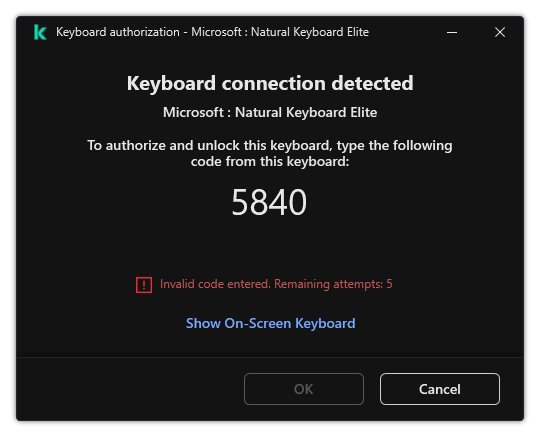
\includegraphics[width=\textwidth]{assets/images/2_loc_screen_kes11_badusb_authorization.png}
		\caption{4-digit PIN verification prompt}
		\label{fig:kaspersky_pin}
	\end{subfigure}
	\caption{Kaspersky Endpoint Security 12.0 BadUSB Prevention interface \cite{kasperskyBadUSB}}
	\label{fig:kaspersky_combined}
\end{figure}

\paragraph{How it works:}
When a USB device enumerates as an HID keyboard, Kaspersky's proprietary kernel driver intercepts the device at Ring 0, blocking all inputs from reaching the OS. As shown in Figure~\ref{fig:kaspersky_pin}, KES displays a prompt containing the peripheral name (e.g., ``Microsoft: Natural Keyboard Elite'') and presents a randomised 4-digit code (\texttt{5840}).

The user must physically read this value from the screen and type it using the newly connected device. Because a malicious microcontroller operates blindly without a camera, it cannot determine the dynamically-generated code and fails the challenge.

\begin{figure}[H]
	\ContinuedFloat
	\centering
	\begin{subfigure}[b]{1\textwidth}
		\centering
		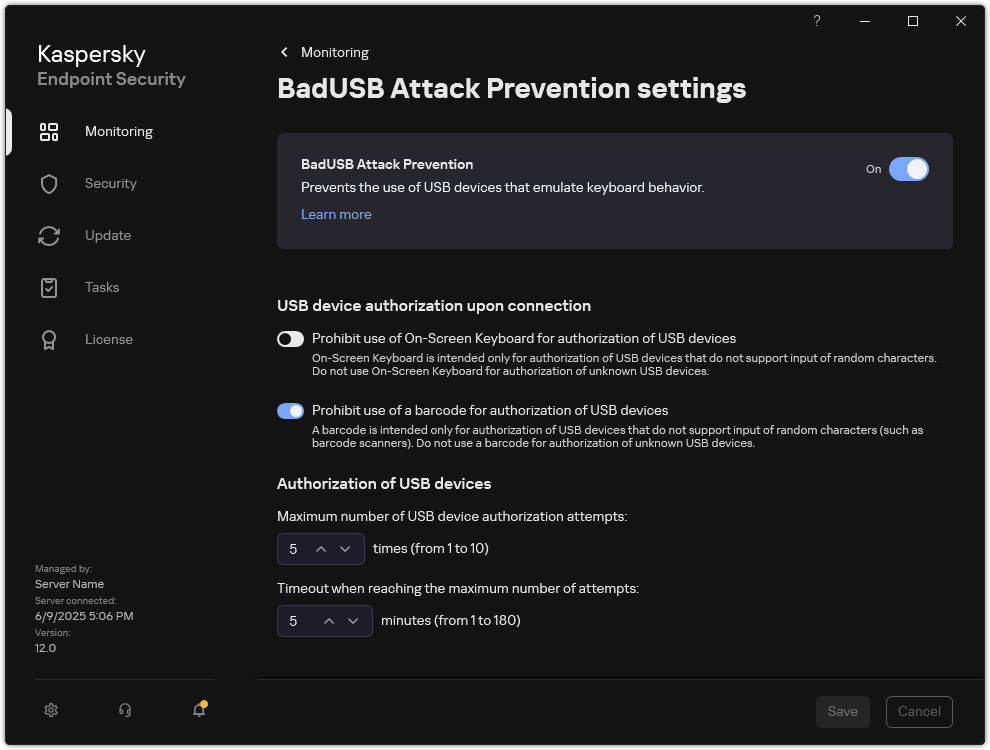
\includegraphics[width=\textwidth]{assets/images/2_loc_screen_kes12_badusb_settings.png}
		\caption{Administrative module configuration}
		\label{fig:kaspersky_settings}
	\end{subfigure}
	\caption[]{(Continued)}
\end{figure}

Figure~\ref{fig:kaspersky_settings} shows the administrative settings panel, detailing the architectural decisions used to harden this captcha-of-sorts:
\begin{itemize}[leftmargin=*, nosep]
	\item \textbf{Anti-automation limit:} To prevent adversaries rapidly brute-forcing the codes, the administrator can choose an attempt ceiling, followed by a mandatory timeout lockout.
	\item \textbf{Restricting assisted bypass:} The console provides a toggle to
	      ``Prohibit use of On-Screen Keyboard for authorization''. Because on-screen keyboards can be driven programmatically, this fallback can be disabled to prevent automated bypass.
	\item \textbf{Barcode authorisation protocol:} Barcode scanners often emulate HID keyboards as they output dynamic strings. To bypass this, a dedicated toggle exists to allow devices to output a pre-determined static string on connection for authorisation.
\end{itemize}

\paragraph{Analysis for \projectNameFormatted :}
\begin{itemize}[leftmargin=*, nosep]
	\item \textbf{Points for inspiration:} The challenge-response model is sound against blind attacks. Intercepting input before they reach the OS also guarantees that zero keystrokes leak, and the anti-brute-force rate limiter provides a robust fail-safe.
	\item \textbf{Points for avoidance:} The operational friction is exceptionally high. Forcing a user to manually type a PIN every single time they plug in an everyday peripheral directly violates \stakeholdersTU's usability needs for presentation clickers. Furthermore, Kaspersky's solution relies entirely on human verification; it contains no heuristic engine to continuously monitor typing speed or variance once a device is approved. Finally, as visible in Figure~\ref{fig:kaspersky_settings} (``Managed by: Server Name''), the module requires a heavyweight, licensed enterprise client-server infrastructure, making it impractical for standalone consumer use.
\end{itemize}

\subsubsection{Reactive Attack Interception (Beamgun)}

Beamgun is an open-source, user-space utility created by security researcher Josh Lospinoso to mitigate BadUSB attacks on Windows workstations \cite{lospinosoBeamgun}.

\begin{figure}[H]
	\centering
	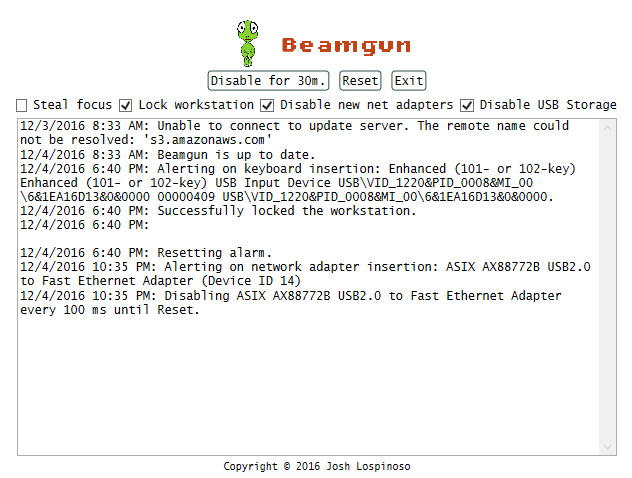
\includegraphics[width=0.8\textwidth]{assets/images/2_loc_screen_beamgun.png}
	\caption{Beamgun user interface and event log during a device insertion event \cite{lospinosoBeamgun}}
	\label{fig:beamgun_ui}
\end{figure}

\paragraph{How it works:}
Beamgun runs as a background process monitoring Windows Plug-and-Play device events (\texttt{WM\_DEVICECHANGE}). Rather than analysing the keystroke timings, it uses blunt countermeasures based on hardware class registration.

As can be seen in the event log in Figure~\ref{fig:beamgun_ui}, when a USB peripheral is plugged in and reports an HID keyboard interface (e.g., \texttt{USB\textbackslash VID\_1220\&PID\_0008}), Beamgun immediately starts various defensive actions:
\begin{itemize}[leftmargin=*, nosep]
	\item \textbf{Workstation locking:} Upon detecting a new keyboard, Beamgun calls the Win32 API to lock the user's active desktop session (shown in the log: ``Successfully locked the workstation''). The rationale is that locking the screen restricts keystrokes, preventing access to the Run prompt, PowerShell, or similar powerful prompts.
	\item \textbf{Focus stealing:} If configured, it aggressively steals window focus away from whichever application is active, with the aim to redirect all keystrokes into an inert window.
	\item \textbf{Network neutralisation:} Sophisticated BadUSB attacks can even emulate USB-to-Ethernet dongles to hijack local traffic. As shown in the log at 10:35~PM, Beamgun continuously disables unrecognised network adapters (e.g., ``ASIX AX88772B USB2.0 to Fast Ethernet Adapter'') every $100\,\text{ms}$.
\end{itemize}

\paragraph{Analysis for \projectNameFormatted :}
\begin{itemize}[leftmargin=*, nosep]
	\item \textbf{Points for inspiration:} Beamgun correctly recognises that BadUSB devices can get extremely complex (e.g., combining HID keyboards with fake network cards). It also proves that useful measures can be implemented in user space without requiring signed kernel drivers.
	\item \textbf{Points for avoidance:}
	      \begin{enumerate}[leftmargin=*, nosep]
		      \item \textbf{User friction:} Calling \texttt{LockWorkStation} every single time an unrecognised keyboard is inserted is extremely annoying for the user. If \stakeholdersTU\ plugs in a presentation clicker, or if \stakeholdersPU's gaming keyboard reconnects after its drivers are updated, their entire desktop is just locked.
		      \item \textbf{Race condition:} Beamgun relies on Windows PnP device notifications, which are asynchronous. Because a microcontroller can transmit its payload within milliseconds of enumeration, an injection script can easily send \texttt{Win+R} and type a command \textit{before} Beamgun obtains the OS message and calls the lock function. It is entirely reactive.
		      \item \textbf{Zero heuristics:} Beamgun also performs no statistical analysis on the keystrokes that are incoming. It treats all keyboard insertions identically, and so fails to distinguish between human typing and faked inputs.
	      \end{enumerate}
\end{itemize}

\subsubsection{OS-Level Gatekeeping (macOS Ventura \& USBGuard)}

Recently, some operating systems have also attempted to solve the BadUSB problem. The most prominent consumer implementation is Apple's ``USB Accessory Security'', introduced in macOS 13 Ventura for Apple Silicon MacBooks \cite{appleAccessorySecurity}.

\noindent
\begin{tabular}{@{}p{0.62\textwidth}@{\hspace{0.04\textwidth}}p{0.34\textwidth}@{}}
	\textbf{How it works:} Rather than letting the OS automatically enumerate new devices, macOS halts the connection at the controller level, restricting newly connected peripherals to power delivery only.

	\smallskip
	As shown in Figure~\ref{fig:macos_prompt}, the OS prompts: ``Allow accessory to connect?''. The data lines remain disabled until approved via the built-in trackpad or an existing keyboard.
	 &
	\vspace{0pt}
	\centering
	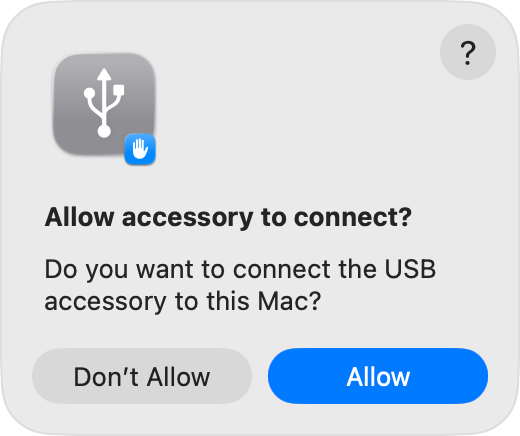
\includegraphics[height=3.1cm, keepaspectratio]{assets/images/2_macos-tahoe-26-allow-accessory-to-connect-dialog.png}
	\vspace{-0.4em}
	\captionof{figure}{macOS prompt \cite{appleAccessorySecurity}}
	\label{fig:macos_prompt}
\end{tabular}

% Restored float specifiers so the image renders normally at the top of Page 22
\begin{figure}[htbp]
	\centering
	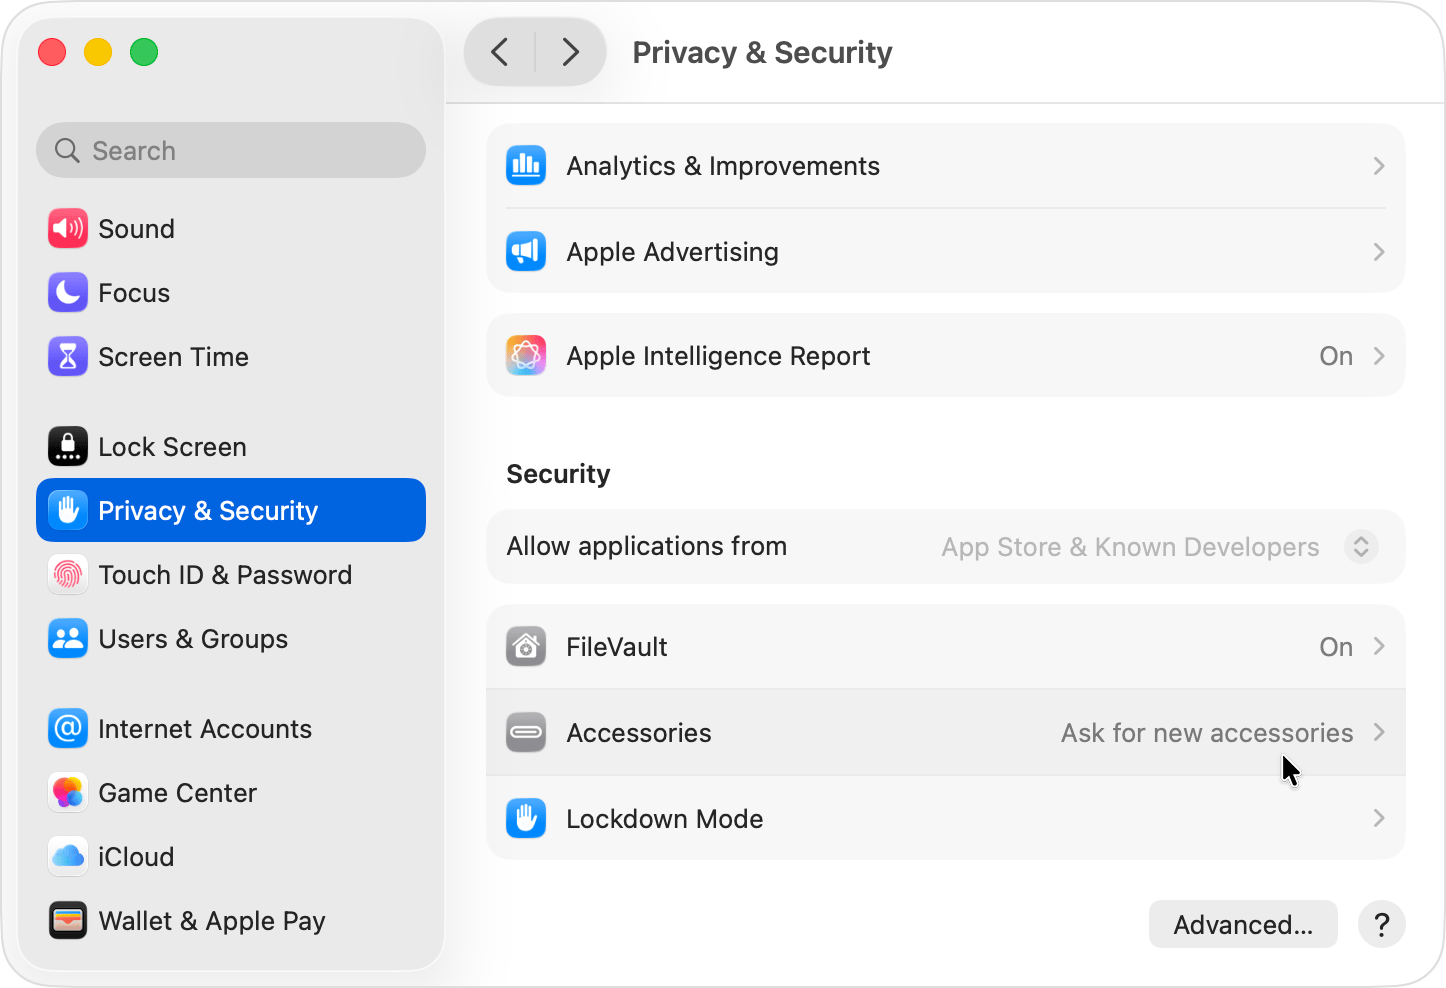
\includegraphics[width=0.8\textwidth]{assets/images/2_macos-tahoe-26-system-settings-privacy-and-security-security-wired-accessories.png}
	\caption{System Settings peripheral access policy options \cite{appleAccessorySecurity}}
	\label{fig:macos_settings}
\end{figure}

% Keep this intro sentence and list together so LaTeX can't split them across pages
\begin{samepage}
	\noindent
	As illustrated in Figure~\ref{fig:macos_settings}, macOS exposes configurable peripheral access policies under \textit{System Settings $\rightarrow$ Privacy \& Security}:
	\begin{itemize}[leftmargin=*, nosep]
		\item \textbf{Ask for new accessories:} Prompts once for new hardware; previously approved devices reconnect without a prompt.
		\item \textbf{Ask every time:} A strict zero-trust policy, prompting on every insertion.
		\item \textbf{Automatically when unlocked:} Approves any device while the session is unlocked, defending only against locked-screen attacks.
	\end{itemize}
\end{samepage}

A comparable implementation in enterprise Linux is \textbf{USBGuard} \cite{usbguardLinux}. It operates as a background daemon that interfaces with the Linux kernel's \texttt{sysfs} device tree (\texttt{/sys/bus/usb/devices/}), using declarative allow/block rules based on device hashes before the kernel binds HID drivers.

\paragraph{Analysis for \projectNameFormatted :}
\begin{itemize}[leftmargin=*, nosep]
	\item \textbf{Points for inspiration:} The user interface in Figure~\ref{fig:macos_prompt} is sleek, and accessible to non-technical users like \stakeholdersTU. Intercepting inputs before data transmission ensures that zero keystrokes get through as well.
	\item \textbf{Points for avoidance:}
	      \begin{enumerate}[leftmargin=*, nosep]
		      \item \textbf{Naive trust model:} Once a user clicks ``Allow'', the accessory is granted unrestricted, permanent access to the OS. There is \textbf{zero continuous behavioural analysis} after approval.
		      \item \textbf{Trivial bypass:} Attackers aware of macOS gatekeeping can just program a delay into their BadUSB payload:
		            \begin{equation}
			            t_{\text{insert}} \xrightarrow{\text{User clicks ``Allow''}} \text{Delay: } 30\,\text{seconds} \xrightarrow{\text{User looks away}} \text{Payload Injected}
		            \end{equation}
		            Because macOS performs no post-approval calculations, the delayed payload can execute completely uninhibited.
		      \item \textbf{Consent fatigue:} Prompting for every single USB cable or flash drive can lead users to blindly click ``Allow'' out of habit, completely nullifying the security benefit.
		      \item \textbf{Proprietary lock-in:} The macOS implementation relies on Apple Silicon hardware controllers, making it unavailable on the more common x86 consumer PCs.
	      \end{enumerate}
\end{itemize}

\subsubsection{Evaluation of Potential Approaches}

In response to the limitations observed in the existing solutions, three development approaches were evaluated to determine how \projectNameFormatted\ should be built:

{\small
\begin{xltabular}{\textwidth}{@{} p{3.2cm} L L @{}}
	\caption{Evaluation of Potential Approaches for \projectNameFormatted} \label{tab:approaches_eval} \\
	\toprule
	\textbf{Approach} & \textbf{Advantages \& Suitability} & \textbf{Disadvantages \& Limitations} \\
	\midrule
	\endfirsthead

	\toprule
	\textbf{Approach} & \textbf{Advantages \& Suitability} & \textbf{Disadvantages \& Limitations} \\
	\midrule
	\endhead

	\bottomrule
	\endlastfoot

	\textbf{Approach 1:}\par Kernel-level driver\par\textit{\footnotesize (Ring 0, C/C++)} &
	\begin{itemize}[leftmargin=*, nosep, wide=0pt, left=0pt]
		\item Absolute control over the USB Request Block (URB) driver stack.
		\item Cannot be bypassed by other malware or tampering.
	\end{itemize} &
	\begin{itemize}[leftmargin=*, nosep, wide=0pt, left=0pt]
		\item Any implementation bugs can cause a Kernel Panic / Blue Screen of Death (BSOD).
		\item 64-bit Windows requires expensive Extended Validation (EV) code-signing certificates.
	\end{itemize} \\
	\addlinespace[0.8em]

	\textbf{Approach 2:}\par High-level language\par\textit{\footnotesize (Python)} &
	\begin{itemize}[leftmargin=*, nosep, wide=0pt, left=0pt]
		\item Rapid development lifecycle and various pre-made statistical packages.
		\item Broad portability across operating systems.
	\end{itemize} &
	\begin{itemize}[leftmargin=*, nosep, wide=0pt, left=0pt]
		\item Garbage collection cycles and runtime interpretation add latency, violating \stakeholdersPU's requirements.
		\item Lacks native Win32 hook primitives.
	\end{itemize} \\
	\addlinespace[0.8em]

	\textbf{Approach 3:}\par Compiled native daemon\par\textit{\footnotesize (C + Win32 API)}\par\textbf{[CHOSEN]} &
	\begin{itemize}[leftmargin=*, nosep, wide=0pt, left=0pt]
		\item Minimal execution footprint and hook latency.
		\item Deterministic memory layouts and no runtime garbage collection pauses.
		\item Direct integration with the Win32 API without third-party libraries.
	\end{itemize} &
	\begin{itemize}[leftmargin=*, nosep, wide=0pt, left=0pt]
		\item Requires manual memory management and strict memory-safety.
		\item Platform-specific Win32 bindings require abstraction for other OS ports.
	\end{itemize} \\
\end{xltabular}
}

\paragraph{Conclusion of Research:}
By combining the pre-execution interception of Kaspersky's approach with the lightweight user-space footprint of Beamgun, \projectNameFormatted\ is designed to fill a distinct gap in consumer-level defence. Adopting \textbf{Approach~3} guarantees that the monitoring daemon satisfies \stakeholdersPU's latency threshold while avoiding the catastrophic system-stability risks of Ring~0 kernel drivers.
